\sectionquestion{TA Questions}

This section is for TAs to put their draft questions into. Please see the qtemplates.tex file for how to format the questions. 


\begin{parts}

\part[0] TODO

\part[20] In class, we applied Maximum Likelihood Estimation to derive an update rule for binary logistic regression. The same process can be used to find parameters for other probabilistic models. In this question, we will apply MLE to a Gaussian clustering problem.

We have a set of data points $x^{(i)} \in \mathbb{R}$ that we know is independently, identically distributed in the same normal distribution. We want to learn the parameters of the true distribution $\mu, \sigma$. To do so, we will use stochastic gradient descent. (In reality, in batch learning, there is a closed form solution to single Gaussian clustering. For the sake of this problem, we will use SGD instead.)

The probability of a data point belonging to the distribution is:
\begin{center}
    \[p(y = 1 | x^{(i)}) = \frac{1}{\sigma \sqrt{2 \pi}} e^{-\frac{1}{2}(\frac{x^{(i)}-\mu}{\sigma})^2}\]
\end{center}
Note: In this problem, a label of 1 means that the point belongs to our distribution. We are assuming that all our data points belong to this same Gaussian distribution. In short, don't worry about $p(y=0 | x)$!
    \noaddpoints % to omit double points count
    \begin{subparts}
    \subpart[10] \textbf{Short answer:} Using the process shown in class, derive an expression for the gradient $\frac{d J(\mu, \sigma)}{d \mu}$ for the SGD update step for the mean, where $J(\thetav)$ is the negative log likelihood of the data. $\sigma, \mu$ are yet unknown, so leave them in the expression.
    \fillwithlines{2em}
    \begin{soln}
    \[p(y = 1 | x, \mu, \sigma) = \frac{1}{2 \pi} e^{-\frac{1}{2}(\frac{x-\mu}{\sigma})^2}\]
    \[\ell(x | \mu, \sigma) = log[\frac{1}{2 \pi} e^{-\frac{1}{2}(\frac{x-\mu}{\sigma})^2}]\]
    \[ = log(\frac{1}{2 \pi}) + (-\frac{1}{2}(\frac{x-\mu}{\sigma})^2)\]
    \[-\ell(x | \mu, \sigma) = -log(\frac{1}{2 \pi}) + \frac{1}{2}(\frac{x-\mu}{\sigma})^2 = J(\mu, \sigma)\]
    \[\frac{d J(\mu, \sigma)}{d \mu} = \frac{\mu - x}{\sigma^2}\]
    \end{soln}
    \begin{qauthor}
    Kevin Liu,
    a. Apply the principle of maximum likelihood estimation (MLE) to learn the parameters of a probabilistic model
    b. Given a discriminative probabilistic model, derive the conditional log-likelihood, its gradient, and the corresponding Bayes Classifier
    \end{qauthor} 
    \subpart[10] \textbf{Numerical answer:} With gradient in hand, you begin training your Gaussian model. You initialize your parameters like so: $\mu = 3, \sigma = 2$. The first point you encounter is $x^{(1)} = 6$. Assume a learning rate of 0.1. What is the new value of $\mu$?
    \begin{tcolorbox}[fit,height=1cm, width=2cm, blank, borderline={1pt}{-2pt}]
    %solution
    \end{tcolorbox}
    \begin{soln}
    Based on the gradient solved from the previous part, we have that
    \[\frac{d J(\mu, \sigma)}{d \mu} = \frac{\mu - x}{\sigma^2} = \frac{3 - 6}{2 ^2} = \frac{-3}{4}\]
    We do one update step with SGD on this single example.
    \[\mu' = \mu - \alpha * \frac{d J(\mu, \sigma)}{d \mu} = 3 - 0.1 * -0.75 = 3.075 \]
    Therefore, our answer is 3.075.
    \end{soln}
    \begin{qauthor}
    Kevin Liu, 2b. Apply stochastic gradient descent (SGD) to optimize a function.
    \end{qauthor}
    \end{subparts}

\part[] A Poisson distribution is a probability distribution that is used to show how many times an event is likely to occur over a specified period. The data set below is about observing how many people died of kidney disease each month in 2020. We observed that the count of death is independent from month to month and follows a Poisson Distribution. What is the estimated $\lambda$ using Maximum Likelihood Estimation?
\begin{center}
    \[f(x) = \frac{\lambda^x}{x!} e^{-\lambda}\]
\end{center}
        \begin{table}[H]
          \centering
        \begin{tabular}{ccccc}
          \toprule
          Month & Number of Death \\ \midrule
          1 & 0\\
          2 & 0\\
          3 & 2\\
          4 & 1\\
          5 & 4\\
          6 & 1\\
          7 & 1\\
          8 & 0\\
          9 & 2\\
          10 & 1\\
          11 & 0\\
          12 & 0\\
          \bottomrule
        \end{tabular}
        \caption{}
        \label{tab:cartdata}
        \end{table}

\begin{tcolorbox}[fit,height=1cm, width=2cm, blank, borderline={1pt}{-2pt}]
    %solution
\end{tcolorbox}
    \begin{soln}
    \[\text{argmax}_{\mathbf{\lambda}} \sum_{i=0}^{N}\log(\frac{\lambda^x_i}{x_i!} e^{-\lambda})\]
    \[\text{argmax}_{\mathbf{\lambda}} \sum_{i=0}^{N} x_i \log\lambda + \sum_{i=0}^{N} (-\lambda)\]
    Taking derivative of the function with respect to $\lambda$:
    \[\frac{1}{\lambda}\sum_{i=0}^{N} x_i - N = 0\]
    \[\lambda = \frac{1}{N}\sum_{i=0}^{N} x_i\]
    The solution will be average of the number of death = 1
    \end{soln}
    
    \begin{qauthor}
    Siyuan Liu, MLE
    \end{qauthor}

\part[] Inspired by the usage of Poisson Distribution to model kidney disease mortality rate, your friend Alice wants to use the MLE of Poisson Distribution to estimate the number of death related to COVID-19. Do you think Alice's approach is reasonable? Why or Why not?
\begin{tcolorbox}[fit,height=1cm, width=15cm, blank, borderline={1pt}{-2pt}]
    %solution
\end{tcolorbox}
    \begin{soln}
    No. It is because COVID-19 cases are not independent from each other.
    \end{soln}
    
    \begin{qauthor}
    Siyuan Liu, MLE
    \end{qauthor}
    
\part[3]
Suppose we cut the normal distribution in half and define the probability density function (pdf) of Right Normal Distribution $RN(\mu,\sigma^2)$ as follows:
\begin{align*}
    f_X(x)=\begin{cases}
    \frac{\sqrt{2}}{\sqrt{\pi}\sigma}\exp\left(-\frac{(x-\mu)^2}{2\sigma^2}\right) &\text{if $x\ge\mu$}\\
    0 &\text{otherwise}
    \end{cases}
\end{align*}
Let $\mathcal{D}=\{1,-1,0\}$ be three iid datapoints sampled from $RN(\mu,\sigma^2)$.
\begin{subparts}
    \subpart[1] Which of the following values of $\mu$ gives the largest likelihood:
    \begin{checkboxes}
         \choice 2
         \choice 0.5
         \choice -0.5
         \choice -2
    \end{checkboxes}
    \begin{soln}
    D
    \end{soln}
    \subpart[2] Compute $\hat{\mu}^{MLE}$. Show your work.\\
    Hint: Since the likelihood is not continuous in $\mu$, some good observations from (a) may be more helpful than differentiation.
    \begin{tcolorbox}[fit,height=1cm, width=15cm, blank, borderline={1pt}{-2pt}]
        %solution
    \end{tcolorbox}
    \begin{soln}
    Observe that if $\mu>\min_{x\in\mathcal{D}}x$, the likelihood is zero so $\hat{\mu}^{MLE}=-1$ gives the largest likelihood.
    \end{soln}
\end{subparts}

\begin{qauthor}
Catherine Cheng, MLE
\end{qauthor}


\part[4]
Suppose $\mathcal{D}=\{x_1, x_2, ... x_n\}$ is sampled from a Laplace distribution That is,  
\begin{align*}
    p(x | \mu)= \frac{1}{2b} e^ {-|x-\mu|/b}
\end{align*}
Note that $b>0$.
\begin{subparts}

    \subpart[1] Compute $\hat{\mu}^{MLE}$. Show your work.\\
    \begin{tcolorbox}[fit,height=3cm, width=15cm, blank, borderline={1pt}{-2pt}]
        %solution
    \end{tcolorbox}
    \begin{soln}
      
\begin{align*}
    \hat{\mu}_{MLE} &= \argmin_\mu -\log\left(p(\Dc|\mu)\right)\\
    &=\argmin_\mu-\log\left( \prod_{1}^{n} \frac{1}{2b} e^ {-|x_i-\mu|/b})\right)\\
    &=\argmin_\theta -\sum_{1}^{n} \log\left( \frac{1}{2b} e^ {-|x_i-\mu|/b}\right)\\
    &=\argmin_\theta -\sum_{1}^{n} {-|x_i-\mu|}\\
    &=\argmin_\theta \sum_{1}^{n} {|x_i-\mu|}\\
    &=mean(x_1, x_2, ... x_n)\\
\end{align*}
  
    \end{soln}
\end{subparts}

\begin{qauthor}
Anoushka Tiwari, MLE
\end{qauthor}



    
    
%%%%% BEGIN JINGYUN'S QUESTION %%%%%

\part[12]
% Inspiration to this problem comes from slide #5 of the following slide deck.
% https://www.cs.ubc.ca/~murphyk/Teaching/CS340-Fall07/NB.pdf
%
\textbf{Poisson Naive Bayes.} Your friend Sergey is given the task of classifying whether a given email is spam ($Y = 1$) or not ($Y = 0$). He has a dictionary of vocabulary that consists of $M$ words. Given an email, he builds feature $X_1, \ldots, X_M$, where $X_m$ is \textit{the number of times} word $m$ in the vocabulary occurs in the email. Confused about how to proceed, Sergey comes to you for help.

Equipped with the knowledge you acquired through 10-301/601, you told Sergey that a good approach to this problem is to design a Naive Bayes Classifier with the following distributions:
\begin{align*}
    Y &\sim \text{Bernoulli}(\phi) \\
    X_m|Y = y &\sim \text{Poisson}(\lambda_{y, m}) \quad (y \in \{0, 1\}; m \in \{1, \ldots, M\}).
\end{align*}

Intrigued, Sergey asks if you can walk through your solution to the problem with him.

\begin{subparts}
    \subpart[2] Assume that the dataset has $N$ samples denoted as $\mathcal{D} = \{(x^{(i)}, y^{(i)})\}_{n=1}^N$, where $x^{(i)} = (x^{(i)}_1, \ldots, x^{(i)}_M)$ are the $M$ features and $y^{(i)} \in \{0, 1\}$ are the labels. Write out the likelihood function of the data $p(\mathcal{D}~|~\phi, \lambda)$.
        \begin{tcolorbox}[fit,height=2cm, width=15cm, blank, borderline={1pt}{-2pt}]
        %solution
        \end{tcolorbox}
        \begin{soln}
            $ p(\mathcal{D}~|~\phi, \lambda) = \prod_{i=1}^N p(y|\phi) \prod_{m=1}^M p(x^{(i)}_m|y^{(i)}, \lambda_{y,m}) \\\phantom{p(\mathcal{D}~|~\phi, \lambda)}= \prod_{i=1}^N \phi^{y^{(i)}} (1-\phi)^{1-y^{(i)}} \prod_{m=1}^M \frac{\lambda_{y^{(i)},m}^{x^{(i)}_m}}{x^{(i)}_m!}e^{-\lambda_{y^{(i)},m}}. $
        \end{soln}
    \subpart[1] Write out the log-likelihood function $\ell(\phi, \lambda)$. In the next 3 parts of the question (starting from this part), you can use the following notations: $N_{y=1} = \sum_{i=1}^N y^{(i)}$; $N_{y=0} = \sum_{i=1}^N (1 - y^{(i)})$; $N_{x_m} = \sum_{i=1}^N x_m^{(i)}$.
        \begin{tcolorbox}[fit,height=2cm, width=15cm, blank, borderline={1pt}{-2pt}]
        %solution
        \end{tcolorbox}
        \begin{soln}
            $ \ell(\phi, \lambda) = N_{y=1}\log \phi + N_{y=0} \log(1-\phi)  \\
            \phantom{\ell(\phi, \lambda)} + \sum_{i=1}^N \sum_{m=1}^M x_m^{(i)} \log(\lambda_{y^{(i)},m}) - \log(x_m^{(i)}!) - \lambda_{y^{(i)},m}. $
        \end{soln}
    \subpart[2] Compute $\hat{\phi}$, the MLE estimate of $\phi$.
        \begin{tcolorbox}[fit,height=2cm, width=15cm, blank, borderline={1pt}{-2pt}]
        %solution
        \end{tcolorbox}
        \begin{soln}
            $\hat{\phi} = N_{y=1} / N.$
        \end{soln}
    \subpart[2] Compute $\hat{\lambda_{y,m}}$, the MLE estimate of $\lambda_{y,m}$.
        \begin{tcolorbox}[fit,height=2cm, width=15cm, blank, borderline={1pt}{-2pt}]
        %solution
        \end{tcolorbox}
        \begin{soln}
            $\hat{\lambda_{y,m}} = N_{x_m} / N.$
        \end{soln}
    \subpart[2] Given a new sample $x = (x_1, \ldots, x_M)$, write out the expression that gives the classification output of the Naive Bayes Classifier. Your answer should be in terms of $\hat{y}$, $\hat{\lambda_{y,m}}$, $x$, and $M$.
        \begin{tcolorbox}[fit,height=2cm, width=15cm, blank, borderline={1pt}{-2pt}]
        %solution
        \end{tcolorbox}
        \begin{soln}
            $\hat{y} = \text{argmax}_{y} \hat{\phi}^y (1-\hat{\phi})^{1-y} \prod_{m=1}^M \lambda_{y,m}^{x_m} e^{-\hat{\lambda_{y,m}}}$. \\
            (Note that the factorial term can be left out of the equation because it is shared for different $y$ values.)
        \end{soln}
    \subpart[1] Sergey is very excited after hearing about your solution. However, he wonders if your proposed algorithm will work if a new email contains words that are not in the vocabulary. Explain your answer to this question.
        \begin{tcolorbox}[fit,height=2cm, width=15cm, blank, borderline={1pt}{-2pt}]
        %solution
        \end{tcolorbox}
        \begin{soln}
            The algorithm will still work in this scenario because the extracted features $x$ won't be affected.
        \end{soln}
    \subpart[2] Sergey wonders whether he should using your Naive Bayes algorithm to his email classification problem or simply use a logistic regression algorithm that takes the same features as input. \textbf{Select all that apply:} which of the following are valid reasons that favors the use of Naive Bayes algorithm over logistic regression?
    \checkboxchar{$\Box$} % change checkbox style locally
    \begin{checkboxes}
     \choice Naive Bayes is faster to train.
     \choice When training data size reaches infinity, Naive Bayes tends to performs better than logistic regression.
     \choice Naive Bayes is more robust to outliers.
     \choice Naive Bayes is more interpretable than logistic regression.
     \choice Naive Bayes makes more realistic assumptions than logistic regression.
     \choice None of the above.
    \end{checkboxes}
    \begin{soln}
    AD.
    Reference: Andrew Ng's paper http://ai.stanford.edu/~ang/papers/nips01-discriminativegenerative.pdf.
    \end{soln}
    
    
\end{subparts}

\begin{qauthor}
Jingyun Yang, Naive Bayes
\end{qauthor}
    
%%%%%  END JINGYUN'S QUESTION  %%%%%

\part[] % To reformat later: label train data plot axes (x1, x2), add bias term, weights to nn figure, redo f(x) plot; numerical-answer boxes for part (b) + (c) 
In this problem, we would like to learn a binary classifier using a neural network. The 2-dimensional training data is plotted as below. 
\begin{center}
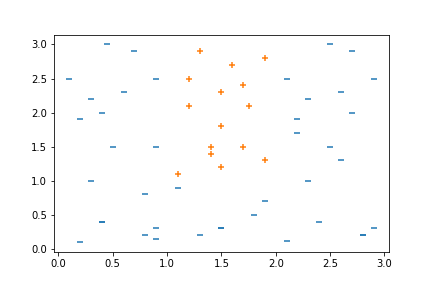
\includegraphics[width=10cm]{figures/plot.png}
\end{center}

The neural network we use will be defined by:

$$y = sign(c + \frac{1}{3} \sum_{i=1}^3 z_i)$$
$$z_i = f (\alpha_{i,1} x_1 + \alpha_{i,2} x_2 + b_i)$$

\bigskip

where $sign(x) = 1$ when $x > = 0$ and $sign(x) = 0$ when $x < 0$.

In the model, $f(x)$ is a linear activation function for the hidden nodes.

\begin{center}
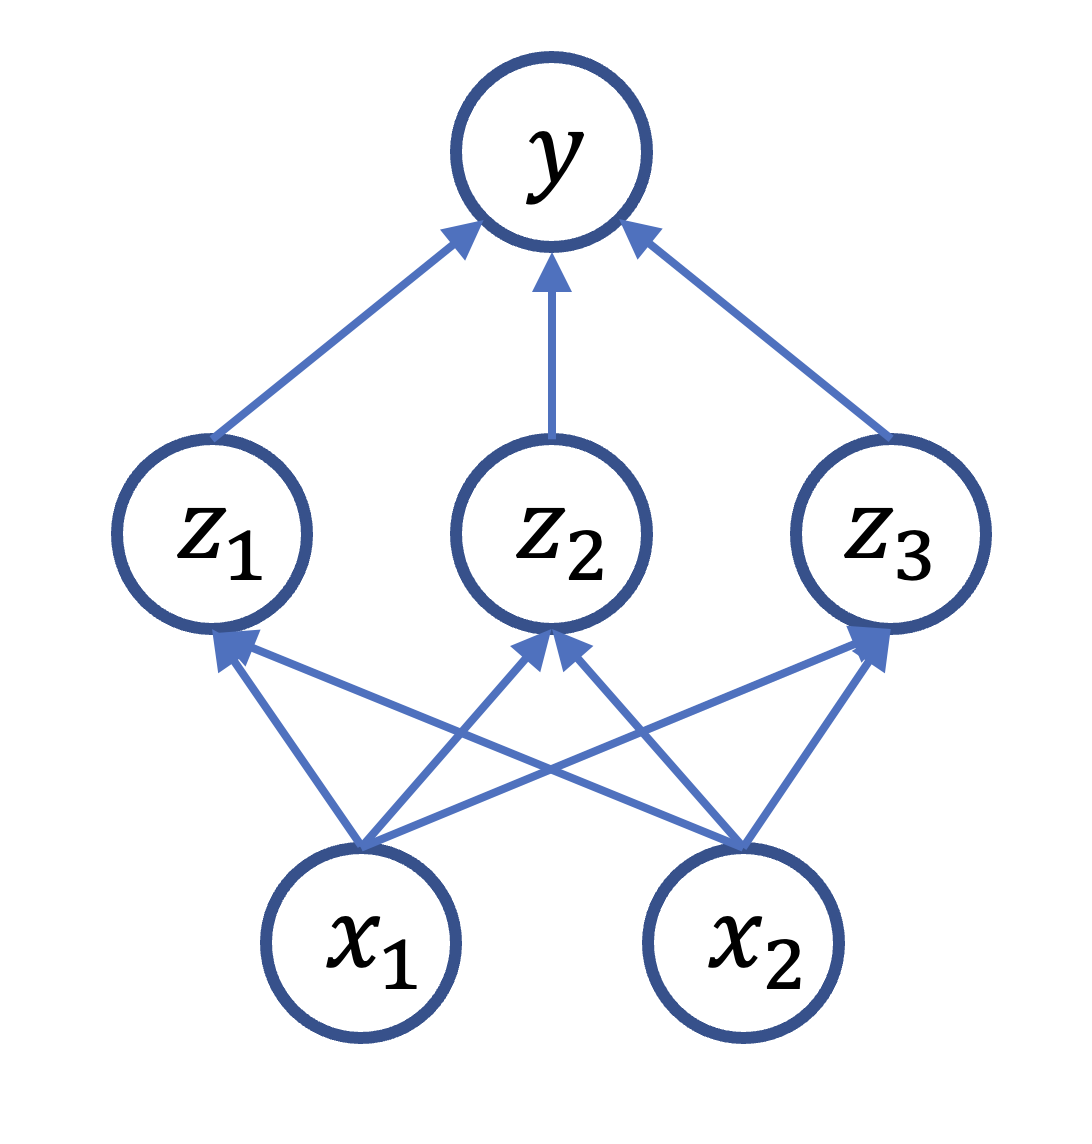
\includegraphics[width=6cm]{figures/nn.png}
\end{center}


\medskip

The function $f(x)$ is shown in the graph below:  

\begin{center}
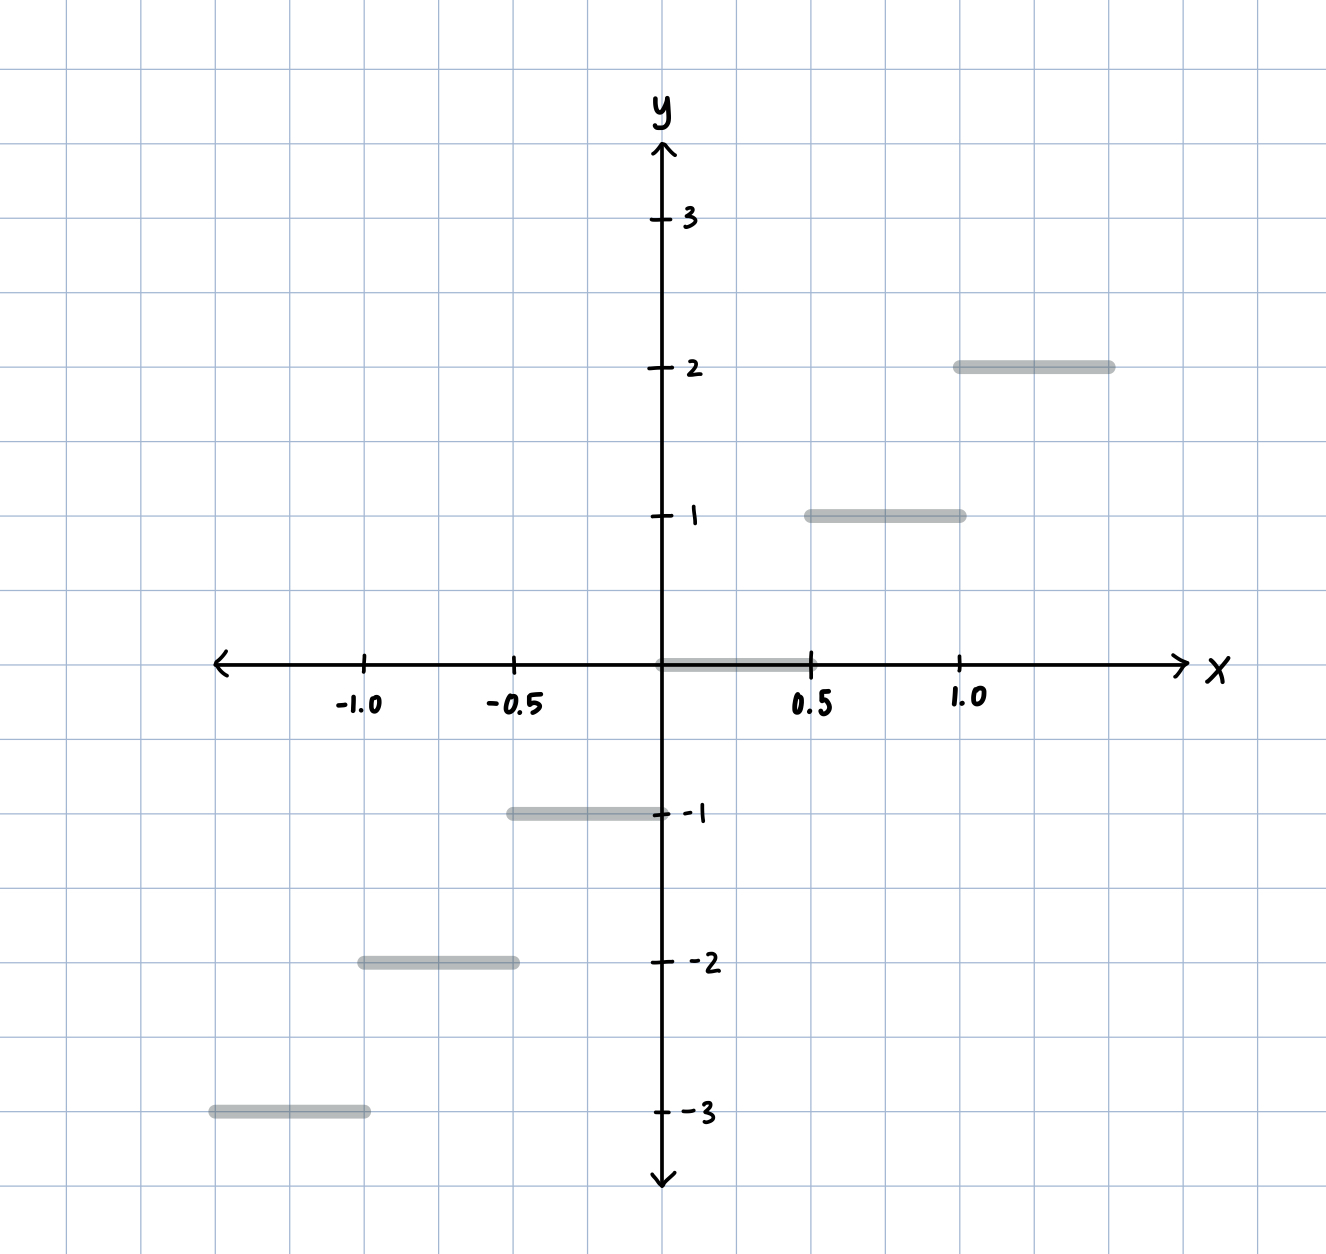
\includegraphics[width=8cm]{figures/step.jpeg}
\end{center}

\begin{subparts}
    \subpart[] The weights $\alpha_{i,j}$'s and $b_i$'s have been learned from the training data so that the training data is perfectly classified. Note, $c$ is another parameter that has been learned to have the value $c = 1$. For simplicity, assume that $\alpha_{i,j} \in \{ -1, 0, 1 \}$ and $b_i$'s are all integers. 
    
    
    In the training data plot, draw the three lines  given by:
    
    (Hint: each line should be parallel to one of the axes in the plot)
    
    (i) $\alpha_{1,1} x_1 + \alpha_{1,2} x_2 + b_1 = 0$
    
    (ii) $\alpha_{2,1} x_1 + \alpha_{2,2} x_2 + b_1 = 0$
    
    (iii) $\alpha_{3,1} x_1 + \alpha_{3,2} x_2 + b_1 = 0$
    
    
    
    
    
    
    \subpart[] Write the weights $\alpha_{i,j}$'s and $b_i$ that are likely to have been learned:
    
    (Hint: think about which direction the normal vector of the line should face)
    
    (i) $\alpha_{1,1} = $
    
    (ii) $\alpha_{1,2} = $
    
    (iii) $b_1 = $
    
    (iv) $\alpha_{2,1} = $
    
    (v) $\alpha_{2,2} = $
    
    (vi) $b_2 = $
    
    (vii) $\alpha_{2,3} = $
    
    (viii) $\alpha_{2,4} = $
    
    (ix) $b_3 = $
    
    \subpart[]
    
    For the following test data points, calculate $y$ using the learned weights and the neural network. (Note, $c = 1$ is given).
    
    (i) $x^{(1)} = [3,0.5]$
    
    (ii) $x^{(2)} = [1.5,2.5]$    
        
\end{subparts}

\begin{soln}
Input solution here.
\end{soln}
\begin{qauthor}
(1) Youngjoo Lee (2) Neural Networks
\end{qauthor}


%% Gopi's Deep Network Question
\part[]
Simon is given a function $f(x, y, z)$, and wants to implement the function as a deep learning network. The function definition is given as below:

\medskip

$$f(x, y, z) \{$$
$$\quad a = k\exp{x}$$
$$\quad b = \frac{1}{\ln{y} + a}$$
$$\quad c = mz + n$$
$$\quad u = \sin{b} + c$$
$$\quad \text{return u}$$
$$\}$$

\medskip

\begin{subparts}
    \subpart[] Draw the computational graph that this function would generate.
    \begin{tcolorbox}[fit,height=5cm, width=15cm, blank, borderline={1pt}{-2pt}]
        %solution
    \end{tcolorbox}
    \begin{soln}
        Solution:
        \begin{center}
            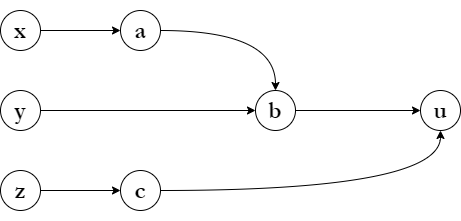
\includegraphics[width=6cm]{figures/backprop.png}
        \end{center}
    \end{soln}
    
    \subpart[] In order for the network to learn, Simon also needs to implement backpropagation. Let $loss$ be the loss between the network's output and the true output. Let $\frac{dloss}{du}$ represent the derivative of the output w.r.t the loss. Given $\frac{dloss}{du}$, Write down the equations Simon needs to implement the backpropagation.
    \begin{tcolorbox}[fit,height=5cm, width=15cm, blank, borderline={1pt}{-2pt}]
        %solution
    \end{tcolorbox}
    \begin{soln}
    \end{soln}
    \begin{qauthor}
        (1) Gopi Krishna (2) Backpropagation
    \end{qauthor}
    
\end{subparts}




%% Ari's Neural Network Question
\part[]
John wants to create a neural network to model a very complex function.
Therefore he chooses to have 1,000 hidden layers with 1,000 hidden nodes each.
For his activation function, he chooses a $f(x)=kx$ for a parameter $k$.
He spends three days training the neural network on a very large
amount of training data through back propagation.
Will his neural network correctly model the unknown function? Why or why not?
\begin{tcolorbox}[fit,height=2.5cm, width=15cm, blank, borderline={1pt}{-2pt}]
%solution
\end{tcolorbox}
\begin{soln}
It will not as he has a linear activation function, so the neural network
will only be able to create a linear decision boundary.
Since the function is very complex, this won't work.
\end{soln}
\begin{qauthor}
Ari Fiorino, Neural Networks
\end{qauthor}
%% Zack's LT Questions
\part[7] Paul is building a classification model for his company. His team lead Duncan wants to be $90\%$ confident that the model is at least $98\%$ accurate. Paul deduces that his model is in the infinite and agnostic case, and presents Duncan with the minimum number of samples in order to guarantee the PAC criterion.
\begin{subparts}
    \subpart[4] A week later, Paul's coworker Jessica points out that the model is actually in the infinite and \emph{realizable} case. If Jessica is right, will the PAC criterion still hold given the number of samples Paul reported to Duncan? Justify your response in 1-2 \emph{concise} sentences.
\begin{tcolorbox}[fit,height=2.5cm, width=15cm, blank, borderline={1pt}{-2pt}]
%solution
\end{tcolorbox}


\begin{soln}
The PAC Criterion will still hold. Since Paul initially thought the hypothesis space was agnostic, Paul's given bound on the number of samples needed is \emph{higher} than if the space is realizable. Thus, though Paul's bound may not be the minimum number of samples to guarantee the PAC criterion, it is still a sufficient number of samples to guarantee it.
\end{soln}
\begin{qauthor}

Zachary Novack, Learning Theory: Testing whether student's know that agnostic bounds are looser than realizable bounds
\end{qauthor}

\subpart[3] Given the disagreement between Paul and Jessica, Duncan decides that now he wants to be $97.5\%$ confident that the model is at least $98\%$ accurate. Based on the number of samples that Paul gave him, how will the minimum number of samples required \emph{approximately change} given the change in confidence?
\begin{checkboxes}
     \choice The minimum number of samples will \emph{decrease} by a factor of approximately 2
     \choice The minimum number of samples will \emph{decrease} by a factor of approximately 4
     \choice The minimum number of samples will \emph{increase} by a factor of approximately 2
     \choice The minimum number of samples will \emph{increase} by a factor of approximately 4
\end{checkboxes}
\begin{soln}
C: Increase by a factor of 2. In either infinite case, the bound is inversely logarithmic in $\delta$. Thus, if $\delta$ decreases by a factor of 4, we would expect the minimum number of samples to increase by a factor of 2.
\end{soln}

\begin{qauthor}
Zachary Novack, Learning Theory: Thinking of SC bounds in terms of $\delta$
\end{qauthor}
\end{subparts}

\part[4] Oscar trains a neural network for image classification, and notices that his model seems to be overfitting to the training data. Because of this, he decides to impose L1 regularization during training. Isaac thinks adding this regularization will increase the VC dimension of the hypothesis space. Is Isaac correct? Justify your response in 1-2 \emph{concise} sentences.
\begin{tcolorbox}[fit,height=2.5cm, width=15cm, blank, borderline={1pt}{-2pt}]
%solution
\end{tcolorbox}
\begin{soln}
Isaac is incorrect. Acceptable answers include reasoning that the VC dimension would decrease or at the most stay the same, not increase, since the model is becoming \emph{less} expressive due to the regularization.
\end{soln}

\begin{qauthor}
Zachary Novack, Learning Theory: VC Dim and Regularization
\end{qauthor}

\part[8] [Chi Gao] Consider the following data set of (x, y):

\begin{center}
    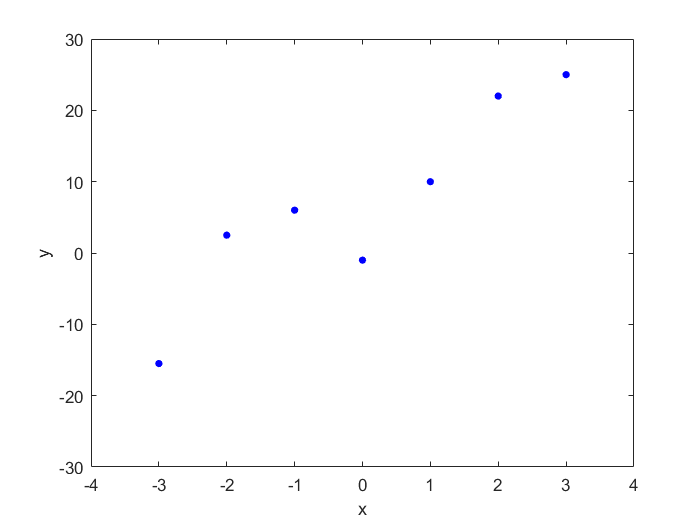
\includegraphics[scale=0.5]{exam2/figures/regularization_question.png}
\end{center}

After some feature engineering work, your friend Pac built a linear regression model:

\begin{align*}
    y = \theta^T\mathbf{x} + b
    \text{  where  }
    \theta = \begin{bmatrix}
        -0.5 \\
        0.5 \\
        5 \\
        2.5
    \end{bmatrix}
    \text{ , }
    \mathbf{x} = \begin{bmatrix}
        x^4 \\
        x^3 \\
        x^2 \\
        x
    \end{bmatrix}
    \text{  and  }
    b = 1.5
\end{align*}

\begin{center}
    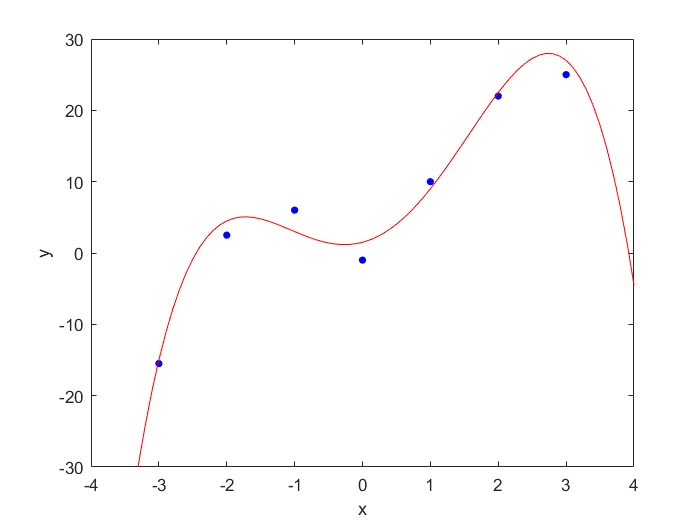
\includegraphics[scale=0.5]{exam2/figures/regularization_model.png}
\end{center}

\begin{subparts} 
    \subpart[2] Pac's model results in poor accuracy during the validation test. In \textbf{one sentence}, describe the potential problem in his feature engineering. 
    
    \begin{tcolorbox}[fit,height=1cm, width=15cm, blank, borderline={1pt}{-2pt}]
    %solution
    \end{tcolorbox}
    
    \begin{soln}
     Pac introduced too many extra dimensions and his model is overfitting.
    \end{soln}
    
    \subpart[3] Based on the problem pointed out in the previous part, which type of the following regularization terms would you introduce to Pac's model to \textbf{completely} remove the problem? Justify your choice and calculate the value of the term you choose. 
    
    \begin{list}{}
     \item\Circle{} L1 regularization
     \item\Circle{} L2 regularization
    \end{list}
    
    \begin{tcolorbox}[fit,height=2cm, width=15cm, blank, borderline={1pt}{-2pt}]
    %solution
    \end{tcolorbox}
    
    \begin{soln}
    Use L1 regularization, since we want to asymptotically remove extra dimensions (by setting them to 0). The result is:
    \begin{equation*}
    \sum|\theta_k| = 0.5 + 0.5 + 5 + 2.5 = 8.5
    \end{equation*}
    \end{soln}
    
    \subpart[3] Suppose the $y$ values of all data points are increased by 1.5 and Pac's model is correspondingly shifted. Would your regularization term in the previous part change? If your answer is "Yes", calculate the change in your regularization term. If "No", justify your answer.
    
    \begin{tcolorbox}[fit,height=3cm, width=15cm, blank, borderline={1pt}{-2pt}]
    %solution
    \end{tcolorbox}
    
    \begin{soln}
    No. Because the purpose of regularization is to control the weights of parameters and reduce unnecessary features. We should not penalize the learning algorithm due to the shift of all data points, and including bias term in the regularization defeats this purpose.
    \end{soln}
\end{subparts}
\begin{qauthor}
Chi Gao, Feature Engineering/Regularization
\end{qauthor}


\part[] Suppose that $10\%$ of the population has diabetes. 


\begin{table}[H]
  \centering
    \begin{tabular}{ |c|c|c|c|  }
    \hline
    \multicolumn{4}{|c|}{Diabetes Distribution} \\
    \hline
    Calories (X) & $<1400$ & $1400-1800$ & $>1800$ \\
    \hline
    diabetes (Y=1) & $20\%$ & $50\%$ & $30\%$ \\
    no diabetes (Y=0) & $10\%$ & $10\%$ & $80\%$ \\
    \hline
    \end{tabular}
    \caption{Conditional Probability Table, where each entry is $P(X|Y)$}
\end{table}



What is the probability that someone has diabetes given that they eat $1400$ to $1800$ calories a day?
\begin{tcolorbox}[fit,height=1cm, width=2cm, blank, borderline={1pt}{-2pt}]
    %solution
\end{tcolorbox}
    \begin{soln}
    $$P(Y=1|X) = \frac{P(X|Y=1)P(Y=1)}{P(X)}=\frac{.5*.1}{.1*.5+.9*.1}=\frac{5}{14}$$
    $$P(Y=0|X) = \frac{P(X|Y=0)P(Y=0)}{P(X)}=\frac{9}{14}$$
    \end{soln}
    
    \begin{qauthor}
    Justin Hsu, Generative Models
    \end{qauthor}

\part Is X independent of Y? 
\begin{tcolorbox}[fit,height=1cm, width=2cm, blank, borderline={1pt}{-2pt}]
    %solution
\end{tcolorbox}
    \begin{soln}
    No. We need to show that $P(X)P(Y)\neq P(X \cap Y)$. Counter Example:
    $$P(Y=1)=.1$$
    $$P(X<1400)=P(X|Y=1)P(Y=1)+P(X|Y=0)P(Y=0)=.1*.2+.9*.1=.11$$
    $$P(X<1400 \cap Y=1) = P(X|Y=1)P(Y=1)=.1*.2=.02$$
    $$.11 * .1 \neq .02$$
    \end{soln}
    
    \begin{qauthor}
    Justin Hsu, Generative Models
    \end{qauthor}

    

\end{parts}


